\section{Introduction}

\subsection{Dimensionality Reduction and Singular Value Decomposition}

In many applications data can be represented as a matrix that defines a mapping
between two feature spaces. As an example a dataset of ratings of users for
movies may be considered. As depicted in Figure~\ref{fig:exmpl_matrix}, such a
dataset can be modeled as a matrix in which each row represents a user, each
column a movie, and each value a rating that a user has given a movie.

\begin{figure}[h]
\centering
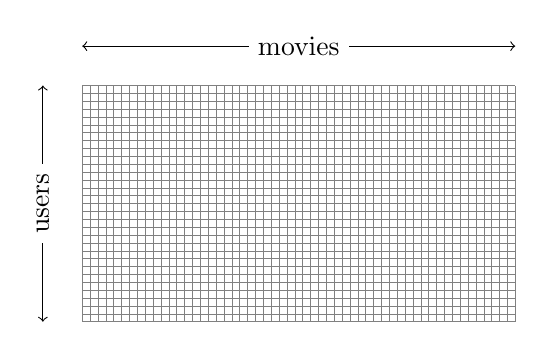
\begin{tikzpicture}
\draw[<->] (0,0.5) -- (0,3.5) node[pos=.5,sloped,fill=white] {users};
\draw[<->] (0.5,4) -- (6,4) node[pos=.5,sloped,fill=white] {movies};
%\draw      (0.5,0.5)  rectangle(6,3.5);
\draw[step=1mm,gray,very thin] (0.4999,0.4999) grid (6,3.5);
\end{tikzpicture}
\caption{Example of a matrix that represents a dataset of ratings from users
for movies}
\label{fig:exmpl_matrix}
\end{figure}

The general goal of such a matrix or vector representation of data is to exploit well known mathematical functions and properties to process the data, which is done by many machine learning and data mining algorithms. However, if at least one feature space is very large, which means in the example that the number of movies or users is very high, the practical application of this approach is hindered. The most obvious reason for this roots in the size of the data, that can get too large as to fit into main memory or as to be processed efficiently. Beyond that a large number of (possibly dependent) dimensions can render mathematical functions useless---especially vector distances, on which important algorithms in machine learning and data mining rely. The latter class of phenomena is grouped under the term \textsl{curse of dimensionality}.

One approach to tackle the aforementioned problems is called \textsl{dimensionality reduction} and aims to syntactically and semantically compress the data's feature spaces by reducing the number of their dimensions. For instance this would mean in our example to compress the number of movies to a more abstract concept like genres as depicted in Figure \ref{fig:exmpl_dr} (in reality, concepts are more fuzzy).

\begin{figure}[h]
\centering
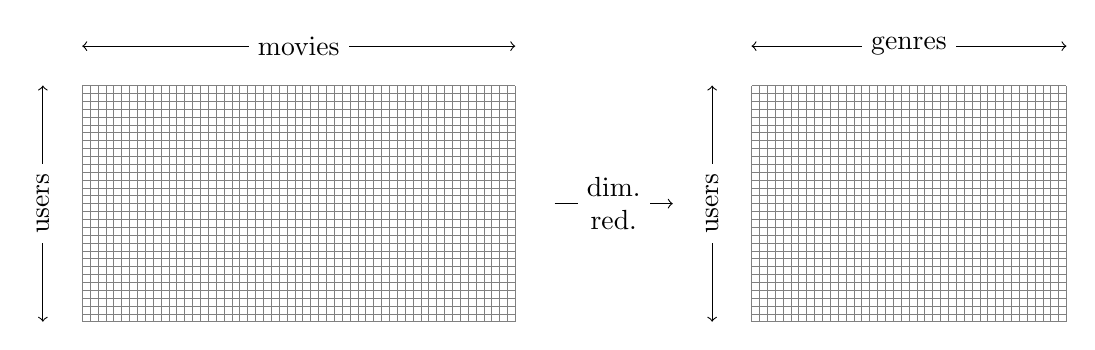
\begin{tikzpicture}
\draw[<->] (0,0.5) -- (0,3.5) node[pos=.5,sloped,fill=white] {users};
\draw[<->] (0.5,4) -- (6,4) node[pos=.5,sloped,fill=white] {movies};
\draw[step=1mm,gray,very thin] (0.4999,0.4999) grid (6,3.5);
\draw[->] (6.5,2) -- (8,2) node[pos=.5,sloped,fill=white, align=center] {dim.
\\ red.};
\draw[<->] (8.5,0.5) -- (8.5,3.5) node[pos=.5,sloped,fill=white] {users};
\draw[<->] (9,4) -- (13,4) node[pos=.5,sloped,fill=white] {genres};
\draw[step=1mm,gray,very thin] (8.9999,0.4999) grid (13,3.5);
\end{tikzpicture}
\caption{Example of dimensionality reduction used to compress the column
feature space from movies to genres}
\label{fig:exmpl_dr}
\end{figure}

This leads to an approximated view of the data, in which a set of movies are
grouped to one or more genres, that are liked or disliked by a set of users.
The approximated data can then be processed more efficiently and sometimes even
more precisely or in a more meaningful way. In \textsl{Latent Semantic
Indexing} for example, a set of documents is indexed by a set of abstract
concepts like topics that are more meaningful to a querying user than a set of
words. The astounding beauty of dimensionality reduction lies in the way it can
be achieved mathematically in an entirely domain agnostic way: With
dimensionality reduction hidden concepts like genres or topics can be
discovered in data that were previously unknown to an investigator. The
abstract concepts like genres or topics are not required to be known in advance
nor is the mapping of concrete feature space dimensions to concepts.

One way of achieving dimensionality reduction is to exploit the
\textsl{Singular Value Decomposition (SVD)} of a matrix. The SVD of a matrix
represents that matrix as a product of three special matrices:

\begin{equation}
	M = U \times \Sigma \times V^T
\end{equation}

$U$ is the basis of the row-feature space and $V$ is the basis of the
column-feature space. So $U$ consists of orthonormal eigenvectors of $M\times
M^T$ and $V$ consists of orthonormal eigenvectors of $M^T\times M$. A
mathematical intuition for this results from building the product of $M$ with
it's transpose and vice versa analog:

\begin{align*}
M \times M^T 	& = (U \times \Sigma \times V^T) \times (V \times \Sigma^T \times
U^T) \\
					& = (U \times \Sigma) \times (\Sigma^T \times U^T) \\
					& = U \times \Sigma^2 \times U^T
\end{align*}

So $U$ and $V$ result from the eigendecompositions of $M\times M^T$ and $M^T\times M$ respectively. $\Sigma$ is a diagonal matrix that holds the corresponding square-rooted eigenvalues in descending order. Figure \ref{fig:svd} gives a more detailed view on the SVD of a matrix $M$. 

\begin{figure}[h]
	\centering
	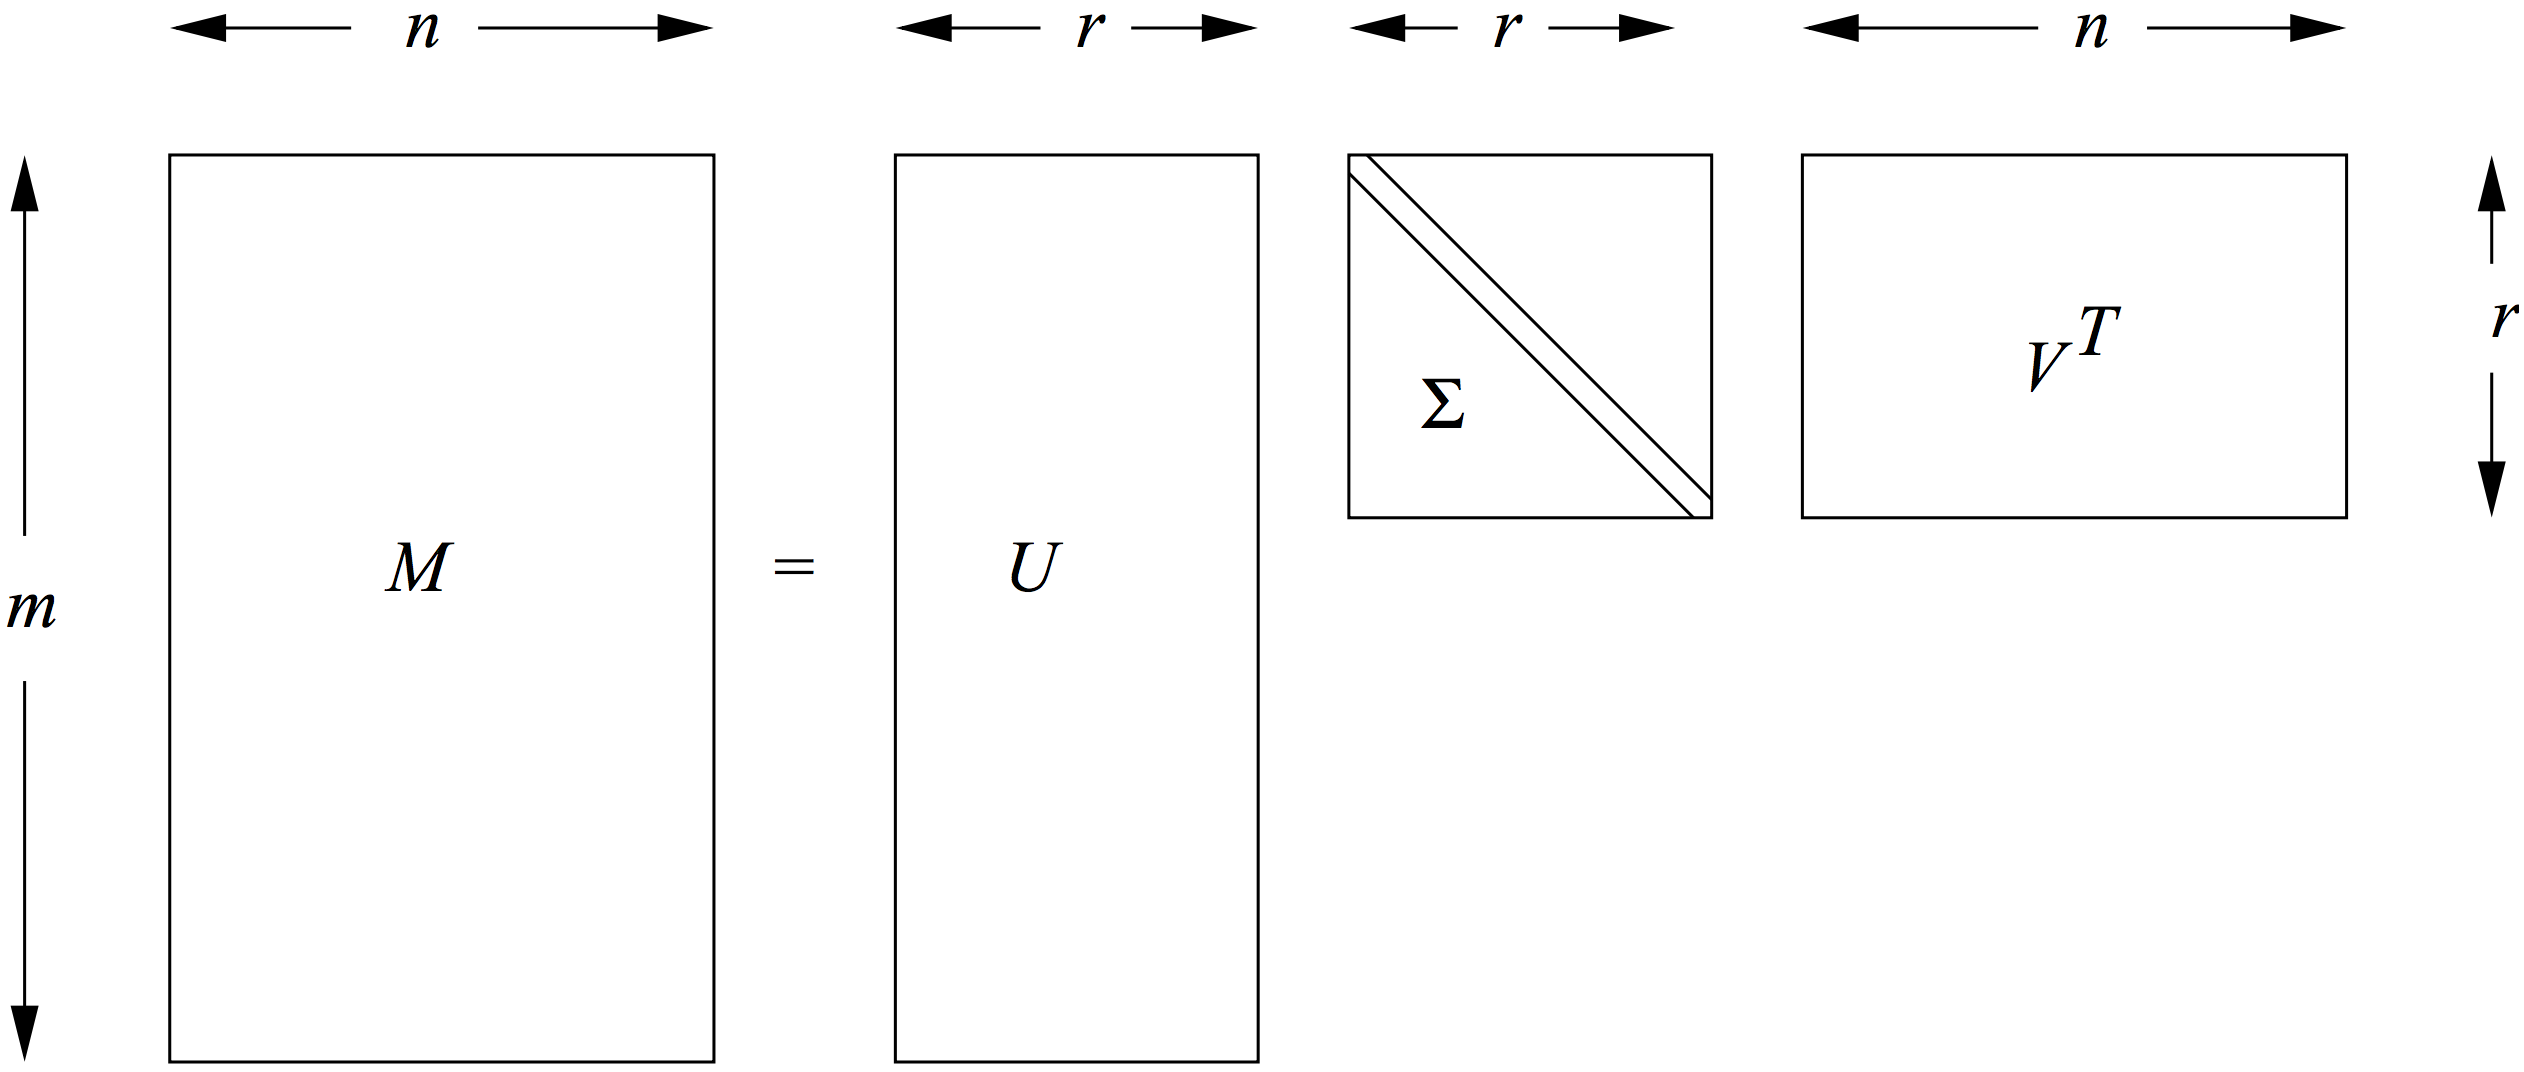
\includegraphics[width=0.8\textwidth]{images/svd_mmds.png}
	\caption{Depiction of the SVD of a matrix $M$}
	\label{fig:svd}
\end{figure}

The actual reduction of dimensions is then performed by dropping least significant eigenvalues of $\Sigma$ along with corresponding eigenvectors in $U$ and $V$ and keeping only the top $k$ one. The resulting matrix in then called the $\text{rank}_k$ approximation of $M$. This works because the column vectors of $U$ and $V$ are normalized and thus do not contribute value or length to a recomposed element. That is entirely done by the eigenvalues of $\Sigma$. By dropping the smallest values of those, a lowest possible approximation error is ensured.

\subsection{The Lanczos Algorithm and Eigendecomposition}
\label{ssec:lanczos_algorithm}

In order to compute the SVD of a matrix, the eigendecompositions of $MM^T$ and $M^T M$ have to be computed:

\begin{align*}
	Eig(MM^T) = (U,\Sigma^2), \;	\;\;	\;\;	\;\;\;	Eig(M^T M) = (V,\Sigma^2)
\end{align*}

This is very expensive if even possible for large matrices, especially when considered that only the top $k$ eigenpairs are kept. The Lanczos algorithm is often used as an auxiliary tool, as it provides the possibility to indirectly compute only the top $k$ eigendecomposition: The Lanczos algorithm takes as input a symmetric and quadratic matrix $A$ (which is $MM^T$ or $M^T M$ in our case) and computes as result a matrix $L$ of Lanczos vectors and a symmetric, tridiagonal auxiliary matrix $T$.

\begin{align*}
	Lanzcos(A) = (L,T) \;\;\;\;\;\;\;\;
	L_{m\times k} = \left ( \vec{l_1}, ... \vec{l_i}, ... \vec{l_k} \right ) \;\;\;\;\;\;\;\;
	T_{k\times k} = \begin{pmatrix}  
\alpha_1 & \beta_2  &          & 0 \\
\beta_2  & \alpha_2 & \ddots   & \\
         & \ddots   & \ddots   & \beta_k \\
0        &          & \beta_k  & \alpha_k \\
\end{pmatrix}
\end{align*}

Because $T$ is symmetric and tridiagonal a traditional eigendecomposition of $T$ is very efficient:

\begin{align*}
	Eig(T) = (Q_T,\Lambda_T)
\end{align*}

The eigenvalues of $A$ are then the same as the one of $T$ ($\Lambda_A = \Lambda_T$) and the eigenvectors of $A$ can be calculated by:

\begin{align*}
	Q_A = L \times Q_T
\end{align*}

As the Lanczos algorithm is the only part in this roadmap that operates on the large initial data, this is the most crucial part that needs to be parallelized. The following listing contains a pseudo code variant of the Lanczos algorithm:

\begin{flalign*}
\texttt{1}\quad &l_1 \leftarrow \, \text{uniformly distributed vector with norm 1} \\
\texttt{2}\quad &l_0 \leftarrow 0 \\
\texttt{3}\quad &\beta_1 \leftarrow 0 \\
\texttt{4}\quad &\textbf{for} \; j = 1,2,\cdots,k-1\\
\texttt{5}\quad &\qquad w_j \leftarrow A l_j\\
\texttt{6}\quad &\qquad \alpha_j \leftarrow  w_j \cdot l_j \\
\texttt{7}\quad &\qquad w_j \leftarrow w_j - \alpha_j l_j   - \beta_j l_{j-1} \\
\texttt{8}\quad &\qquad \textbf{for}\; i = 1, 2, \cdots,j-2 \\
\texttt{9}\quad &\qquad \qquad w_j \leftarrow w_j - \left(w_j \cdot l_i\right) l_i \\
\texttt{10}\quad &\qquad \textbf{endfor} \\
\texttt{11}\quad &\qquad \beta_{j+1} \leftarrow \left\| w_j \right\|  \\
\texttt{12}\quad &\qquad l_{j+1} \leftarrow w_j / \beta_{j+1}  \\
\texttt{13}\quad &\textbf{endfor} \\
\texttt{14}\quad &w_k  \leftarrow A v_k \\
\texttt{15}\quad &\alpha_k \leftarrow  w_k \cdot v_k
\end{flalign*}
 
As depicted above the Lanczos algorithm is an \textsl iterive algorithm that computes in each step $\alpha_j$,~$l_{j+1}$~and~$\beta_{j+1}$ given $\l_{j-1}$,~$l_{j}$~and~$\beta_{j}$ from the previous step. 

